\documentclass[conference]{IEEEtran}
\IEEEoverridecommandlockouts

\usepackage{cite}
\usepackage{amsmath,amssymb}
\usepackage{graphicx}
\usepackage{booktabs}
\usepackage{tabularx,array}
\usepackage{url}
\usepackage[hidelinks]{hyperref}

\graphicspath{{figures/}}
\newcommand{\R}{R^2}

\begin{document}

\title{Music Emotion Recognition with Pretrained Audio Embeddings on DEAM\\[0.3em]
\large Progress Report}

\author{\IEEEauthorblockN{Can Y\"uzbey, Cem \"Ozkul, Efe Kumru, Emir Ceylan}
\IEEEauthorblockA{CS 415 Introduction to Deep Learning, Group 21, Sabanc\i\ University, Istanbul, Turkey\\
\{can.yuzbey, cem.ozkul, efe.kumru, emir.ceylan\}@sabanciuniv.edu}}

\maketitle

\begin{abstract}
We predict static valence and arousal for the 1{,}744 clips of DEAM. Following
the instructor's feedback, this report covers the data audit, an artist-grouped
10-fold protocol, the openSMILE baseline and a frozen MERT comparison. The audit revealed two
undocumented defects in the 2013 part of DEAM: swapped static valence/arousal
labels and openSMILE features computed on the full song instead of the rated
excerpt. After correcting both, an SVR reaches $\R=0.38$ (valence) and $0.69$
(arousal) on artist-disjoint folds. We also show that per-clip listener
disagreement is barely measurable with 10 raters, which clarifies what a
variance head can represent. A heteroscedastic head on openSMILE matches the
constant-variance reference only as a seed ensemble, and its learned variance
adds a small error signal for valence. With the same ridge head, MERT
raises $\R$ to $0.56$/$0.75$ (valence/arousal), better in 10 of 10 folds.
\end{abstract}

%======================================================================
\section{Problem and Motivation}
%======================================================================
We predict two continuous emotion scores per music clip, \emph{valence}
(negative to positive) and \emph{arousal} (calm to energetic). Such scores
support emotion-aware music discovery. The task is hard for two reasons:
labelled data are scarce (DEAM has 1{,}744 rated 45\,s
clips~\cite{aljanaki2017}), and listeners disagree. Our aims, in the order
requested in the feedback, are (i) to show that a frozen pretrained encoder
(MERT~\cite{li2024mert}, later also a general-audio encoder) beats
hand-crafted openSMILE features~\cite{eyben2010} with the same regression
head, and (ii) to establish precisely what the
variance of a heteroscedastic head trained with Gaussian negative
log-likelihood (NLL) represents.

%======================================================================
\section{Related Work}
%======================================================================
DEAM comes from the MediaEval ``Emotion in Music'' tasks (2013--2015) and
provides static and dynamic valence and arousal ratings together with
openSMILE features~\cite{aljanaki2017}. Regression with support vector
regression (SVR) on such hand-crafted features is the usual baseline; on DEAM,
Cheuk \emph{et al.}~\cite{cheuk2020} report $\R\approx0.32$ (valence) and
$0.64$ (arousal) for an SVR on openSMILE features, and improve on it with a
triplet network. Pretrained encoders let us fit only a small head on DEAM.
MERT~\cite{li2024mert} is self-supervised on music and reports strong emotion
regression results with frozen features and a small probing head. Results on
random splits may partly reflect artist or production cues, so we evaluate on
artist-grouped folds.

A heteroscedastic network predicts a mean and a variance and is trained with
the Gaussian NLL. Seitzer \emph{et al.}~\cite{seitzer2022} show that under
plain NLL the samples a model predicts badly receive relatively small updates,
which can leave the mean poorly fitted, and they introduce $\beta$-NLL to
counter this. For MER, Watcharasupat \emph{et
al.}~\cite{watcharasupat2025} find that models learn the mean rating but not
how much listeners disagree; we examine why.

%======================================================================
\section{Data}
%======================================================================
We use the 1{,}744 45\,s excerpts of the 2013 (744) and 2014 (1{,}000)
campaigns; the 58 full songs of 2015 follow a different protocol and are
excluded. Each clip has static valence and arousal ratings on a 1--9 scale
from 10--20 raters (median 10, 187 raters in total) and dynamic ratings at
2\,Hz. We rescale the mean rating by $(\mu-5)/4$ to $[-1,1]$ and the listener
standard deviation by $s/4$. After the correction in Sec.~\ref{sec:res},
valence and arousal correlate at $r=0.61$ (Fig.~\ref{fig:dis}a).

\begin{figure}[t]
\centering
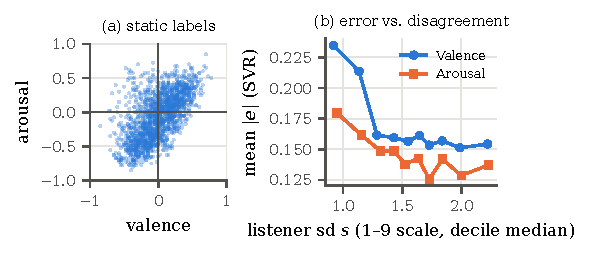
\includegraphics[width=0.92\columnwidth]{fig_labels_disagreement}
\caption{(a) Corrected labels. (b) SVR error per decile of listener spread $s$.}
\label{fig:dis}
\end{figure}

%======================================================================
\section{Design Decisions}
%======================================================================
Table~\ref{tab:deviations} summarises all changes to the proposal; the main
ones are explained below.

% DRAFT deviation table (Efe): changes since the approved proposal, each with
% its reason. Needs \usepackage{booktabs,tabularx} in the preamble.
\begin{table*}[t]
\centering
\caption{Deviations from the approved proposal and their justification.}
\label{tab:deviations}
\footnotesize
\begin{tabularx}{\textwidth}{@{}p{2.6cm}XXp{2.2cm}@{}}
\toprule
\textbf{Aspect} & \textbf{Proposal} & \textbf{Now, and why} & \textbf{Trigger} \\
\midrule
Meaning of $\sigma$ &
$\sigma$ predicted by the NLL head expected to track listener disagreement (H2). &
$\sigma$ is defined as the predicted error of the model on the \emph{mean} rating
(model error plus averaging noise $\approx s^2/n$), not the spread of individual
listeners. $\rho(\sigma,s)$ is kept only as a descriptive analysis. H2 is split
into H2a (calibration, $\sigma$ vs.\ actual error), H2b (how measurable $s$ is)
and H2c (a head trained on individual ratings, after the report). &
Instructor feedback; Watcharasupat \emph{et al.}~\cite{watcharasupat2025} \\
Individual ratings &
Not considered. &
The data audit found per-rater static ratings (10--20 raters per clip, 187 raters),
which enables reliability ceilings now and explicit modelling of the rating
distribution (H2c) later. &
Instructor feedback; data audit \\
Split protocol &
One artist-disjoint 70/15/15 split, three seeds, bootstrap over test songs. &
Artist-grouped, quadrant-stratified 10-fold CV; fold $k{+}1$ is validation.
Every clip is tested exactly once, so uncertainty analyses use all 1{,}744
out-of-fold predictions instead of $\approx$262, and models are compared by
paired per-fold differences. &
Small dataset; \cite{bouthillier2021} \\
Success thresholds &
Fixed $R^2$ targets (e.g.\ C1: $R^2_V\geq0.30$, $R^2_A\geq0.60$; C2: $R^2_V\geq0.45$, $R^2_A\geq0.68$). &
C1 becomes a sanity check reported with its spread, not a pass/fail gate. The
primary H1 criterion is relative: the pretrained encoder must beat openSMILE
\emph{with the same head} on both dimensions. &
Instructor feedback (thresholds optimistic under artist-disjoint CV) \\
Same-head comparison &
SVR on openSMILE vs.\ MLP on MERT. &
Ridge and MLP heads are trained on both openSMILE and MERT so that the
representation effect is not confounded with the head; SVR is reported as an
additional baseline. &
Methodological \\
openSMILE excerpt &
DEAM features used as supplied. &
For the 744 clips of 2013 the supplied feature files cover the \emph{full song}
(up to 585\,s) while audio and ratings cover a 45\,s excerpt. Features are now
cropped to the excerpt using the segment start in the 2013 metadata (offsets
verified against the audio energy). &
Found during baseline work \\
2013 static labels &
Labels used as supplied. &
For the 744 clips of 2013 the static valence and arousal columns are swapped
relative to the dynamic annotations ($r\approx0.95$ crossed vs.\ $\approx0.57$
matched; 2014 is consistent) and to loudness. They are swapped back. &
Found during baseline work \\
2015 full songs &
Secondary out-of-distribution test set (58 songs). &
Dropped: different annotation protocol and only 5 raters per song. &
Scope \\
Scope of the report &
PANNs, fine-tuning and ensembles in weeks 3--5. &
PANNs, random-init MERT (null model), layer probe and LP-FT moved after the
report, following the instructor's ordering of priorities. &
Instructor feedback \\
\bottomrule
\end{tabularx}
\end{table*}


\textbf{Meaning of $\sigma$.} As the feedback noted, a variance fitted to the
\emph{mean} rating $\bar y_i$ of $n_i$ listeners is not the variance between
listeners. With $\mu_i$ the population mean and $f(x_i)$ the prediction,
\begin{equation}
\mathbb{E}[(\bar y_i - f(x_i))^2] = (\mu_i - f(x_i))^2 + s_i^2/n_i ,
\label{eq:sigma}
\end{equation}
i.e.\ model error plus averaging noise; listener spread $s_i$ enters only
divided by $n_i\approx10$. We therefore evaluate $\sigma$ as a predictive
uncertainty (calibration, rank correlation with $|e|$) and treat its relation
to $s$ as descriptive only. Since per-rater ratings exist, a head trained on
individual ratings is planned as a direct model of listener spread.

\textbf{Protocol.} Instead of one 70/15/15 split we use artist-grouped,
quadrant-stratified 10-fold cross-validation (seed 415); for test fold $k$,
fold $k{+}1$ is validation. Every clip is tested once, models are compared by
paired per-fold tests, and no artist appears in two folds. As the feedback
warned that fixed thresholds are optimistic, H1 is now decided relatively:
MERT must beat openSMILE \emph{with the same head} (ridge, then an MLP). We
report, per dimension, $\R$, RMSE (on the $[-1,1]$ and the 1--9 scale),
Pearson $r$ and the concordance correlation coefficient
$\mathrm{CCC}=2\rho s_y s_{\hat y}/(s_y^2+s_{\hat y}^2+(\bar y-\bar{\hat y})^2)$,
which also penalises bias and scale errors. For $\sigma$ models we add the
Gaussian NLL, the coverage of 68\,\% and 95\,\% intervals (PICP) and
Spearman $\rho(\sigma,|e|)$. All metrics come from one shared script that reads
prediction files in a common format.

\textbf{Representations.} openSMILE: mean and standard deviation of DEAM's 260
frame-level descriptors over the excerpt (520-d). MERT-v1-95M~\cite{li2024mert}: nine 5\,s
windows at 24\,kHz (eight for the 9 clips shorter than 45\,s), all 13 layers cached, layer chosen on validation.

\textbf{Variance stability.} The heteroscedastic MLP bounds $\sigma$ softly,
$\sigma=\sigma_{\min}+(\sigma_{\max}-\sigma_{\min})\,\mathrm{sigmoid}(z)$ with
$\sigma_{\min}=0.01$ and $\sigma_{\max}=2\,\mathrm{sd}(y_{\text{train}})$,
avoiding hard clamps that kill gradients. The mean is warmed up with MSE before
switching to $\beta$-NLL~\cite{seitzer2022} ($\beta=0.5$; $\beta=0$ as comparison); early stopping
and model selection use the plain validation NLL, not the $\beta$-NLL loss; and the share
of $\sigma$ near either bound is logged, with $>5\,\%$ flagged as unstable.
The reference is a constant $\sigma$ equal to the validation RMSE.

%======================================================================
\section{Experiments and Results}
\label{sec:res}
%======================================================================
\begin{table}[t]
\centering
\caption{openSMILE baselines, mean $\pm$ SD over 10 test folds.}
\label{tab:baseline}
\footnotesize
\setlength{\tabcolsep}{3pt}
\begin{tabular}{@{}llcccc@{}}
\toprule
Head & Dim & $R^2$ & RMSE & RMSE$_{1\text{--}9}$ & CCC \\
\midrule
Ridge & V & 0.372$\pm$0.079 & 0.216$\pm$0.017 & 0.865$\pm$0.068 & 0.563$\pm$0.070 \\
 & A & 0.671$\pm$0.061 & 0.189$\pm$0.017 & 0.756$\pm$0.068 & 0.806$\pm$0.041 \\
SVR & V & 0.379$\pm$0.075 & 0.215$\pm$0.012 & 0.859$\pm$0.049 & 0.565$\pm$0.063 \\
 & A & 0.693$\pm$0.045 & 0.183$\pm$0.013 & 0.731$\pm$0.051 & 0.822$\pm$0.029 \\
\midrule
Ridge (random split) & V & 0.395$\pm$0.046 & 0.215$\pm$0.008 & 0.859$\pm$0.034 & 0.579$\pm$0.042 \\
 & A & 0.677$\pm$0.036 & 0.189$\pm$0.010 & 0.757$\pm$0.042 & 0.810$\pm$0.020 \\
SVR (random split) & V & 0.414$\pm$0.047 & 0.211$\pm$0.009 & 0.845$\pm$0.035 & 0.599$\pm$0.033 \\
 & A & 0.698$\pm$0.031 & 0.183$\pm$0.009 & 0.732$\pm$0.034 & 0.823$\pm$0.020 \\
\bottomrule
\end{tabular}
\end{table}


\textbf{Audit and split.} A scripted audit confirmed that all 1{,}744 clips
have valid labels, an audio file and an openSMILE file. For one clip (ID 1968)
the averaged arousal differed from the rater mean by 0.62 and was replaced by
it. After normalising names there are 898 artists (1--23 songs each; 67 appear
in both years). The fold file passes an integrity test: each clip appears
once and no artist appears in two folds. Folds hold 134--215 clips, and the
largest deviation of a fold's quadrant share from the overall share is 0.10.

\textbf{Defect 1: swapped 2013 labels.} A first baseline gave $\R_A=0.29$ on
2013 but $0.69$ on 2014. Comparing static labels with the time-averaged dynamic
annotations of the same clips (Fig.~\ref{fig:swap}) shows that in 2013 static
valence matches dynamic \emph{arousal} ($r=0.96$) and vice versa ($0.95$),
while in 2014 the matching dimensions agree ($0.91$/$0.94$). Loudness confirms
this. We swap the 744 clips back.

\textbf{Defect 2: full-song features.} For 2013 the supplied openSMILE files
cover the whole song (up to 585\,s) while audio and ratings cover a 45\,s
excerpt. We crop them using the segment start in the metadata, verified on 21
clips by locating the excerpt's energy curve inside the full-song features
(all within 0.5\,s). Fig.~\ref{fig:fixes} and Table~\ref{tab:batch} show the
effect: cropping improves both dimensions, and after the label fix the gap
between the batches closes. (Valence drops after the fix because, before it,
``valence'' on 2013 was in fact the easier arousal target.)


\begin{figure}[t]
\centering
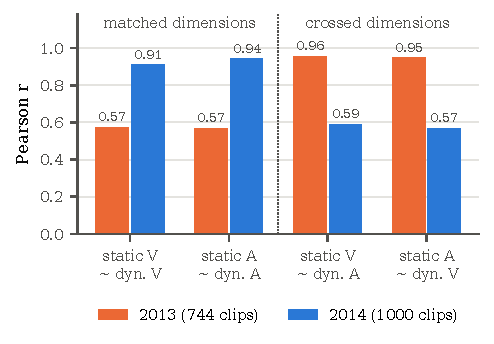
\includegraphics[width=0.92\columnwidth]{fig_va_swap}
\caption{Correlation of static labels with time-averaged dynamic annotations.
In 2013 the crossed dimensions agree: valence and arousal are swapped.}
\label{fig:swap}
\end{figure}

\begin{figure}[t]
\centering
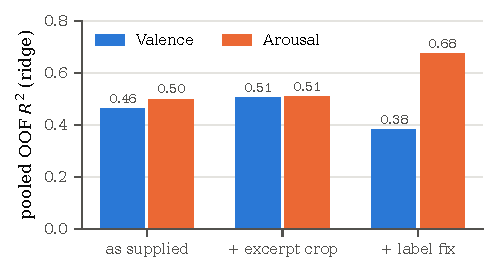
\includegraphics[width=0.92\columnwidth]{fig_data_fixes}
\caption{Pooled out-of-fold $\R$ of ridge with the data as supplied, after
cropping the 2013 features, and after also fixing the 2013 labels.}
\label{fig:fixes}
\end{figure}

\begin{table}[t]
\centering
\caption{SVR $\R$ by batch before/after the label fix.}
\label{tab:batch}
\footnotesize
\begin{tabular}{@{}lcccc@{}}
\toprule
 & \multicolumn{2}{c}{supplied labels} & \multicolumn{2}{c}{corrected} \\
\cmidrule(lr){2-3}\cmidrule(l){4-5}
Batch ($n$) & $\R_V$ & $\R_A$ & $\R_V$ & $\R_A$ \\
\midrule
2013 (744)  & 0.61 & 0.29 & 0.37 & 0.65 \\
2014 (1000) & 0.38 & 0.69 & 0.43 & 0.74 \\
\bottomrule
\end{tabular}
\end{table}



\begin{figure}[t]
\centering
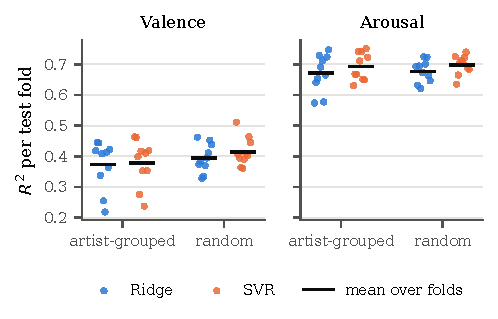
\includegraphics[width=0.92\columnwidth]{fig_baseline_folds}
\caption{Per-fold test $\R$ of the baselines on artist-grouped and random folds.}
\label{fig:folds}
\end{figure}

\textbf{openSMILE baseline.} Hyperparameters were chosen per fold and
dimension on validation RMSE (ridge: 25 values of $\alpha$ in $[10^{-1},10^5]$;
SVR: $C$, $\gamma$, $\epsilon$ grid), and the model was refit on the training
folds (Table~\ref{tab:baseline}, Figs.~\ref{fig:folds}--\ref{fig:scatter}). The SVR
reaches $\R=0.38/0.69$, consistent with the $0.32/0.64$ reported for an SVR by~\cite{cheuk2020}. Their subset (1{,}724 songs) and split differ from ours, and the paper does not state whether the split separates artists, so this comparison is indicative only.
It beats ridge on arousal (8/10 folds, Wilcoxon $p=0.049$) but not on valence.
Random folds raise $\R_V$ by 0.035 but $\R_A$ by only 0.005, so artist
leakage mainly inflates valence. The noise ceiling of the mean rating is
$0.79/0.85$; averaging noise alone explains about 35\,\% (valence) and
50\,\% (arousal) of the SVR's squared error, so a better representation has
clear room to help, especially for valence, whose predictions are also
compressed towards the centre (Fig.~\ref{fig:scatter}).

\textbf{MERT ridge.} With the same ridge head and folds, MERT-v1-95M reaches
$\R=0.56\pm0.07$/$0.75\pm0.03$ (Table~\ref{tab:baseline}), versus $0.37$/$0.67$ for openSMILE ridge:
$\Delta\R=+0.191$/$+0.083$, better in 10/10 folds on both dimensions (Wilcoxon $p=0.002$);
against openSMILE SVR, $+0.185$/$+0.061$, again 10/10. Layer and $\alpha$ were chosen jointly
per fold and dimension on validation (layers 3--8, mostly 6--7); this search (13 layers
$\times$ 25 $\alpha$) is wider than openSMILE's $\alpha$-only search. Random folds raise
MERT $\R$ by 0.027/0.011, similar to openSMILE ridge (0.023/0.006).

\begin{figure}[t]
\centering
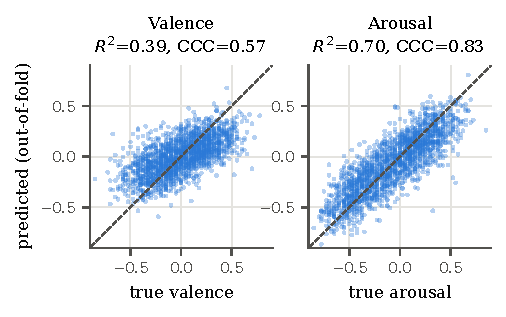
\includegraphics[width=0.92\columnwidth]{fig_baseline_scatter}
\caption{Out-of-fold SVR predictions for all 1{,}744 clips (artist-grouped folds).}
\label{fig:scatter}
\end{figure}

\textbf{Listener disagreement.} Split-half reliability (500 random 5/5 rater
splits, corrected to 10 raters) is high for the mean rating ($0.79$/$0.85$)
but near zero for the listener standard deviation $s$ ($0.00$/$0.04$) and low ($0.21$/$0.13$)
after removing rater bias and scale. Moreover, model error is
\emph{negatively} related to $s$ (Spearman $-0.15$/$-0.10$, $p<10^{-4}$;
Fig.~\ref{fig:dis}b). Clips near the scale centre have more disagreement
(on a bounded scale a mean near the ends forces a small spread;
$\rho(|\mu|,s)=-0.23/-0.30$), while extreme clips are hardest to predict
because regression shrinks towards the centre. With the rater-adjusted $s$ the
correlation vanishes ($0.00/-0.03$). A $\sigma$ that tracks the model's error, as
Eq.~\ref{eq:sigma} implies, therefore can track
disagreement only weakly, which is consistent with the finding of~\cite{watcharasupat2025};
the main limit is the low reliability of $s$.



\textbf{Heteroscedastic head on openSMILE.} The constant-$\sigma$
reference is already calibrated on average (PICP$_{68}\approx0.68$,
PICP$_{95}\approx0.95$; NLL $-0.11$/$-0.24$ for ridge) and by construction has
$\rho(\sigma,|e|)=0$, so the heteroscedastic head must improve NLL and
error ranking to be useful. We trained it on the corrected labels and the
artist-grouped folds with the stabilisation of Sec.~IV ($\beta$-NLL, $\beta\in\{0,0.5\}$,
5 seeds), and score it with the same shared script as the baselines
(Table~\ref{tab:hetero}, Figs.~\ref{fig:cal}--\ref{fig:sig}). Variance was stable:
in none of the 10 runs (2 values of $\beta$, 5 seeds) did a fold have more than
5\,\% of its $\sigma$ near either bound (in fact 0\,\%).

A \emph{single} head does not beat the reference. At $\beta=0$ it reaches
$\R=0.33\pm0.01$/$0.65\pm0.00$ (mean $\pm$ SD over seeds), below ridge, and it
is over-confident (intervals too narrow: PICP$_{95}=0.92$/$0.93$, NLL $-0.06$/$-0.19$ vs.\ $-0.11$/$-0.24$).
$\beta=0.5$ is worse still ($\R=0.29$/$0.63$, NLL $0.02$/$-0.12$), i.e.\ in
our setting it did not improve accuracy. The \emph{5-seed ensemble}, combined
as in deep ensembles~\cite{lakshminarayanan2017} (mean of the member means;
variance = mean member variance plus variance of the means),
closes the gap: $\R=0.375$/$0.679$, PICP$_{68}=0.66$/$0.70$,
PICP$_{95}=0.95$/$0.96$, NLL $-0.135$/$-0.267$. Against the ridge reference its NLL is
better on valence in 8 of 10 folds (Wilcoxon $p=0.014$) and not significantly
on arousal ($p=0.38$); against the SVR reference it is better on valence (9/10 folds,
$p=0.010$) and equal on arousal.
Its $\sigma$ ranks errors: $\rho(\sigma,|e|)=0.17$/$0.14$ (Fig.~\ref{fig:sig}), whereas the constant reference has $0$.

Ensembling alone also improves the mean and the interval, so we separate
the two effects. As a control we gave the same ensemble mean the best possible constant
$\sigma$ per fold (the test RMSE itself, which favours the control). On valence the
learned $\sigma$ still lowers NLL by $0.017$ (8/10 folds, $p=0.014$), which is
most of the $0.026$ gain over ridge. On arousal the learned $\sigma$ adds only
$0.008$ ($p=0.32$), so the arousal improvement comes from ensembling, not from
heteroscedasticity. The ensemble's
valence NLL gain over both references survives Holm correction over the four
comparisons ($p=0.041/0.039$; arousal $p=0.75$). Most of it is due to the learned
$\sigma$ (oracle control, $p=0.014$ uncorrected), so the learned variance carries a
suggestive error signal for valence and none we can demonstrate for arousal. With listener spread it is only weakly related
($\rho(\sigma,s)=0.06$/$0.07$; $0.11$/$0.08$ with rater-adjusted $s$), as expected from Eq.~\ref{eq:sigma}
and the low reliability of $s$. These results use openSMILE only. The MLP settings were fixed, not tuned on validation
(hidden width 128, dropout 0.2, learning rate $10^{-3}$, weight decay $10^{-4}$, 15 warm-up
and up to 60 NLL epochs, patience 10, batch size 32), so its comparison with the tuned ridge reference
mixes head and tuning.

\begin{table}[t]
\centering
\caption{Heteroscedastic head vs.\ the constant-$\sigma$ reference on openSMILE, artist-grouped folds (seed ensemble of 5). Mean $\pm$ SD over the 10 test folds; $\rho$ is Spearman on all pooled out-of-fold predictions. Ideal PICP is $0.68$/$0.95$; for the references $\rho\approx0$ because $\sigma$ is constant within each fold.}
\label{tab:hetero}
\footnotesize
\setlength{\tabcolsep}{2.5pt}
\begin{tabular}{@{}llcccccc@{}}
\toprule
Model & D & $R^2\uparrow$ & PICP$_{68}$ & PICP$_{95}$ & NLL$\downarrow$ & $\rho(\sigma,|e|)$ & $\rho(\sigma,s)$ \\
\midrule
Ridge, const. $\sigma$ & V & 0.372$\pm$0.079 & 0.673$\pm$0.051 & 0.949$\pm$0.022 & $-$0.109$\pm$0.078 & $\approx$0 & $\approx$0 \\
 & A & 0.671$\pm$0.061 & 0.680$\pm$0.058 & 0.949$\pm$0.025 & $-$0.236$\pm$0.101 & $\approx$0 & $\approx$0 \\
\midrule
SVR, const. $\sigma$ & V & 0.379$\pm$0.075 & 0.673$\pm$0.034 & 0.952$\pm$0.018 & $-$0.116$\pm$0.058 & $\approx$0 & $\approx$0 \\
 & A & 0.693$\pm$0.045 & 0.668$\pm$0.061 & 0.943$\pm$0.026 & $-$0.270$\pm$0.083 & $\approx$0 & $\approx$0 \\
\midrule
Hetero. MLP, $\beta{=}0$ & V & 0.375$\pm$0.079 & 0.664$\pm$0.041 & 0.948$\pm$0.017 & $-$0.135$\pm$0.056 & 0.17 & 0.06 \\
 & A & 0.679$\pm$0.039 & 0.700$\pm$0.039 & 0.962$\pm$0.019 & $-$0.267$\pm$0.046 & 0.14 & 0.07 \\
\midrule
Hetero. MLP, $\beta{=}0.5$ & V & 0.353$\pm$0.087 & 0.656$\pm$0.044 & 0.939$\pm$0.022 & $-$0.115$\pm$0.065 & 0.17 & 0.04 \\
 & A & 0.671$\pm$0.042 & 0.682$\pm$0.039 & 0.949$\pm$0.028 & $-$0.249$\pm$0.064 & 0.11 & 0.04 \\
\bottomrule
\end{tabular}
\end{table}


\begin{figure}[t]
\centering
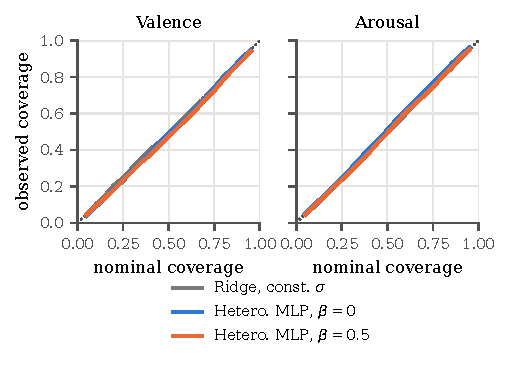
\includegraphics[width=0.92\columnwidth]{fig_hetero_calibration}
\caption{Reliability of the predictive intervals on pooled out-of-fold predictions
(seed ensembles for the heteroscedastic heads). The dotted line is perfect calibration.}
\label{fig:cal}
\end{figure}

\begin{figure}[t]
\centering
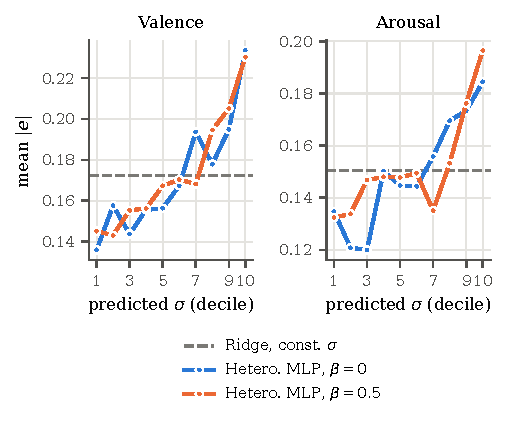
\includegraphics[width=0.92\columnwidth]{fig_hetero_sigma}
\caption{Mean absolute error per decile of predicted $\sigma$. A constant-$\sigma$
model is flat by construction (dashed: its overall mean $|e|$ is the reference level).}
\label{fig:sig}
\end{figure}

%======================================================================
\section{Summary and Next Steps}
%======================================================================
We audited the data, built and verified an artist-grouped 10-fold protocol,
corrected two defects in DEAM 2013, established the openSMILE baseline
($\R=0.38/0.69$, CCC $=0.57/0.82$), showed that MERT with the same ridge head reaches $\R=0.56/0.75$, quantified the artist effect, and showed
that listener disagreement is barely measurable, which fixes how $\sigma$ will
be interpreted. On openSMILE, the heteroscedastic head is stable, but a single
head is worse than the constant-$\sigma$ reference; a 5-seed ensemble matches it on
accuracy, is calibrated, and has a lower NLL on valence (owed mostly to the learned $\sigma$; on
arousal the gain comes from ensembling), while its $\sigma$ ranks errors only weakly
($\rho(\sigma,|e|)\approx0.15$). Next we will (1) train an MLP on MERT and repeat the heteroscedastic head on MERT;
(2) check whether the valence gain survives on MERT; and
(3) then add a general-audio encoder and a head trained on individual ratings.

\bibliographystyle{IEEEtran}
\bibliography{refs}

\end{document}
